\documentclass{article}

\usepackage[top=2cm, bottom=1.5cm, right=1.5cm, left=2cm]{geometry}
\usepackage{graphicx}
\usepackage{hyperref}

\usepackage{caption}
\usepackage{subcaption}

\author{Ana Larissa da Silva Dias \and Cassio Trindade Batista \and Edwin Jair Rueda \and Erick Modesto Campos}
\title{Disaster at St. Himark!\\VAST 2019 Mini Challenge 3}

\begin{document}
\maketitle

\begin{section}{Question}
\subsection{Characterize conditions across the city}
There appears to have occurred three earthquakes, but the first seems to
have started at 2~PM of the first day (April 6th), as
can be seen at the heatmap of Figure~\ref{fig:eq_start_heat}. The heatmap is
divided by a time interval of one hour and by neighbourhood location. It was
generated by considering a list of keywords that were tweeted and are similar in 
meaning (synonyms) and are directly related to the word ``earthquake''. The list 
is: ``\emph{shake}'', ``\emph{shudder}'', ``\emph{vibrate}'', ``\emph{wobble}'',
``\emph{tremor}'', ``\emph{tremble}'', ``\emph{quaver}'', ``\emph{quiver}'',
``\emph{hazard}'', ``\emph{disaster}'', ``\emph{destruction}'', and
``\emph{rubble}''.

To ensure the heatmap is providing a reliable information, a horizontal bar
chart, shown in Figure~\ref{fig:eq_start_hbar}, was used from 1:30~PM to 
3:00~PM. It counts isolated 
words and discards words such as adverbs, pronouns, adjectives, articles and 
some nouns and verbs that were considered to be useless such as ``anyone'',
``make'', ``know'', ``food'', ``hate'', etc. Then the Porter Stemmer from the
\texttt{nltk} package was used to clip the words by its invariant parts (word 
root), and that root was further reduced to 4-chars only. A heat-like colormap
from blue to red was also included to enhance frequency distinction. 

The bar chart shows some interesting other words such as ``\emph{feel}'',
``\emph{hear}'', ``\emph{report}'' apart from the keywords aforementioned, in
which ``\emph{earthquake}'' is the most frequent one in accordance with the red
color.

\begin{figure}[!h]
    \centering
    \begin{subfigure}[!h]{0.95\textwidth}
        \centering
        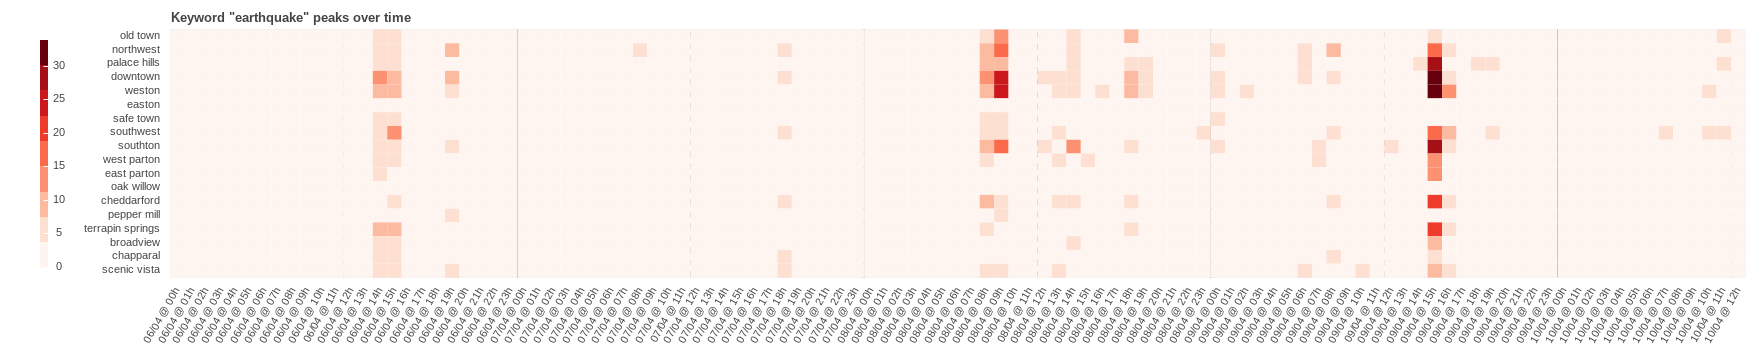
\includegraphics[width=1.00\textwidth]{figs/eq_start_heat.png}
        \caption{Heatmap considering cluster of similar keywords (synonyms)}
        \label{fig:eq_start_heat}
    \vspace{12pt}
    \end{subfigure}
    \begin{subfigure}[!h]{0.95\textwidth}
        \centering
        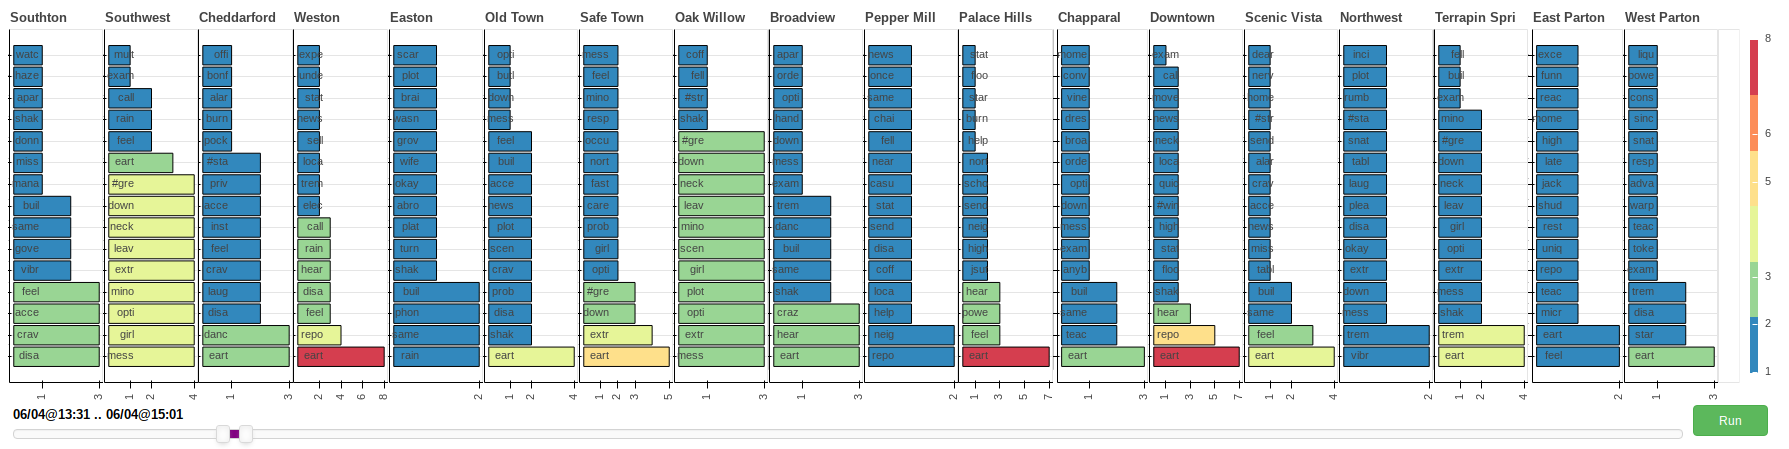
\includegraphics[width=1.00\textwidth]{figs/eq_start_hbar.png}
        \caption{Bar chart with blue-to-red colormap considering frequency of
        words from Apr 6th 1:00~PM to Apr 6th 3~PM.}
        \label{fig:eq_start_hbar}
    \end{subfigure}
    \caption{Earthquake start}
    \label{fig:eq_start}
\end{figure}

\subsection{How resources should be allocated 5h after the earthquake?}

\begin{figure}[!h]
    \centering
    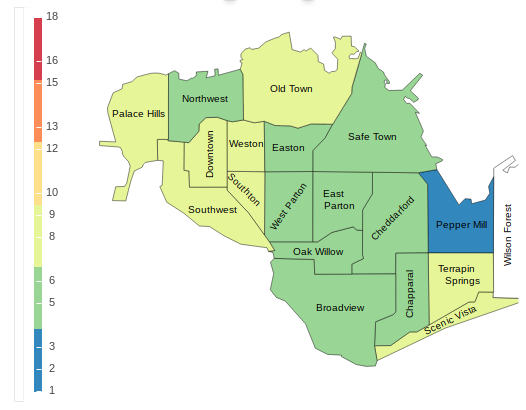
\includegraphics[width=0.30\textwidth]{figs/cond_5h/cond_5h_svg.png}
    \label{fig:map_5h}
    \caption{St. Himark's map 5h after the first earthquake.}
\end{figure}

Figure~\ref{fig:eq_cond_5h} shows the heatmap per keyword in a five-hour-time 
interval from 2:00~PM to 6:59~PM. The top shows 3 blank graphs for the keywords
``building'', ``medical'', and ``road'', which means these resources do not 
appear to be requested by any neighbourhood. On the other hand, the 3 graphs at
the bottom show the number of mentions for keywords related to 
``sewer and water'', ``power'', and ``rain''. 

\begin{figure}[!h]
    \centering
    \begin{subfigure}[!h]{0.32\textwidth}
        \centering
        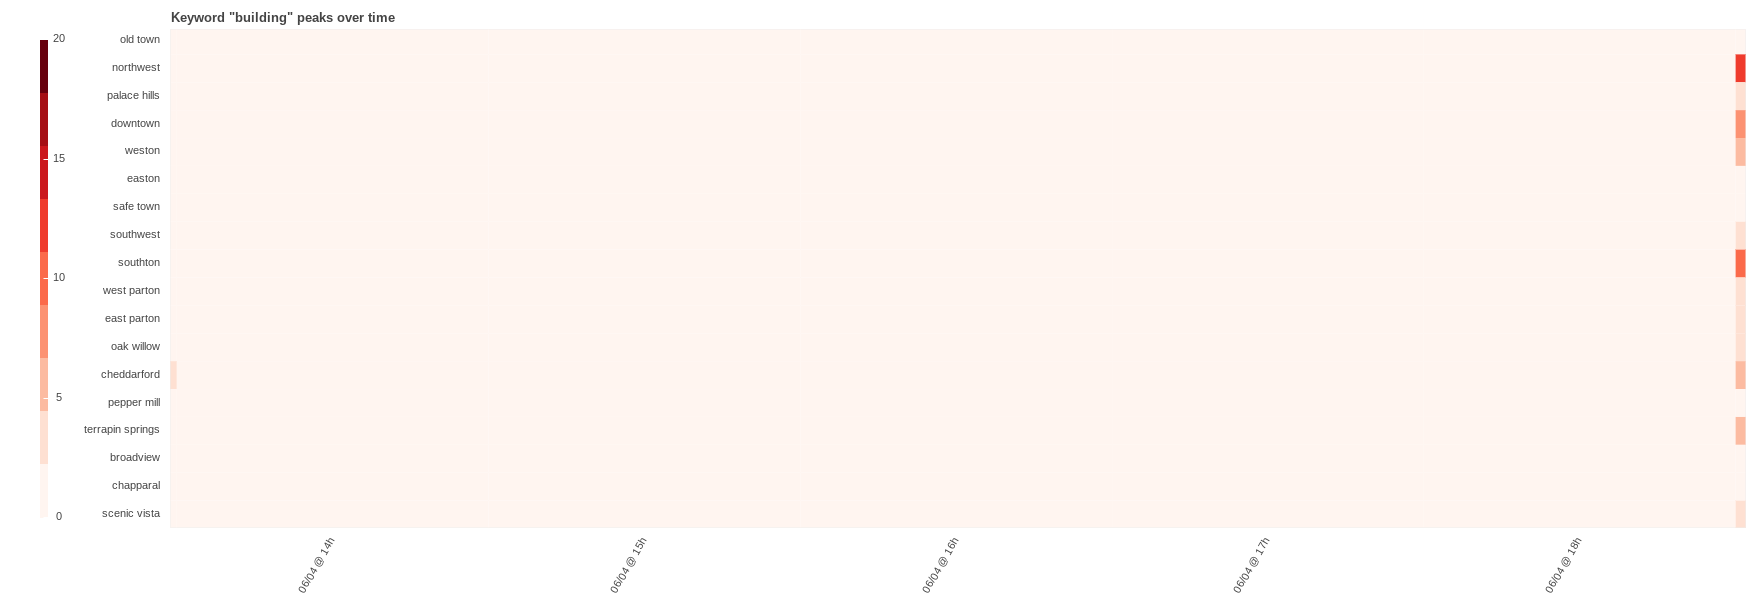
\includegraphics[width=1.00\textwidth]{figs/cond_5h/cond_5h_build.png}
        \caption{Building}
    \end{subfigure}
    \begin{subfigure}[!h]{0.32\textwidth}
        \centering
        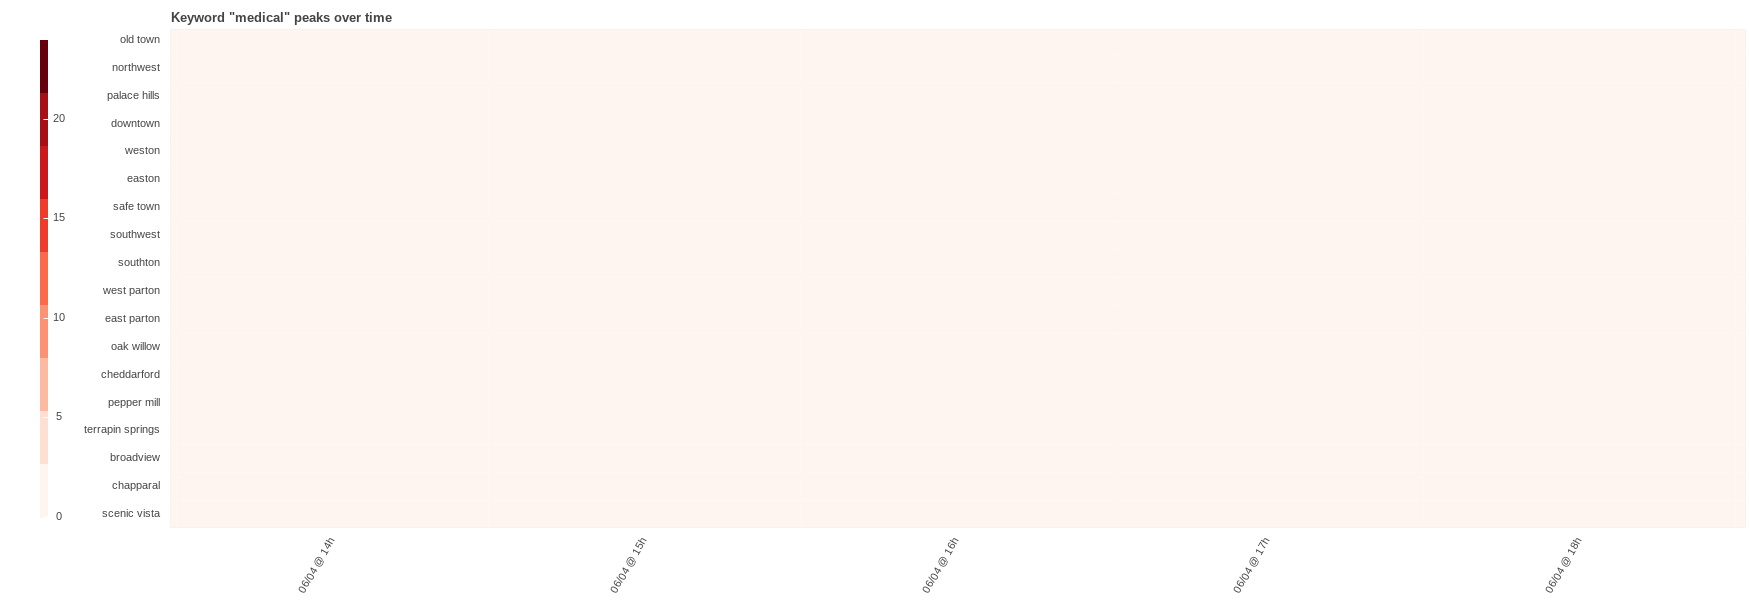
\includegraphics[width=1.00\textwidth]{figs/cond_5h/cond_5h_medical.png}
        \caption{Medical}
    \end{subfigure}
    \begin{subfigure}[!h]{0.32\textwidth}
        \centering
        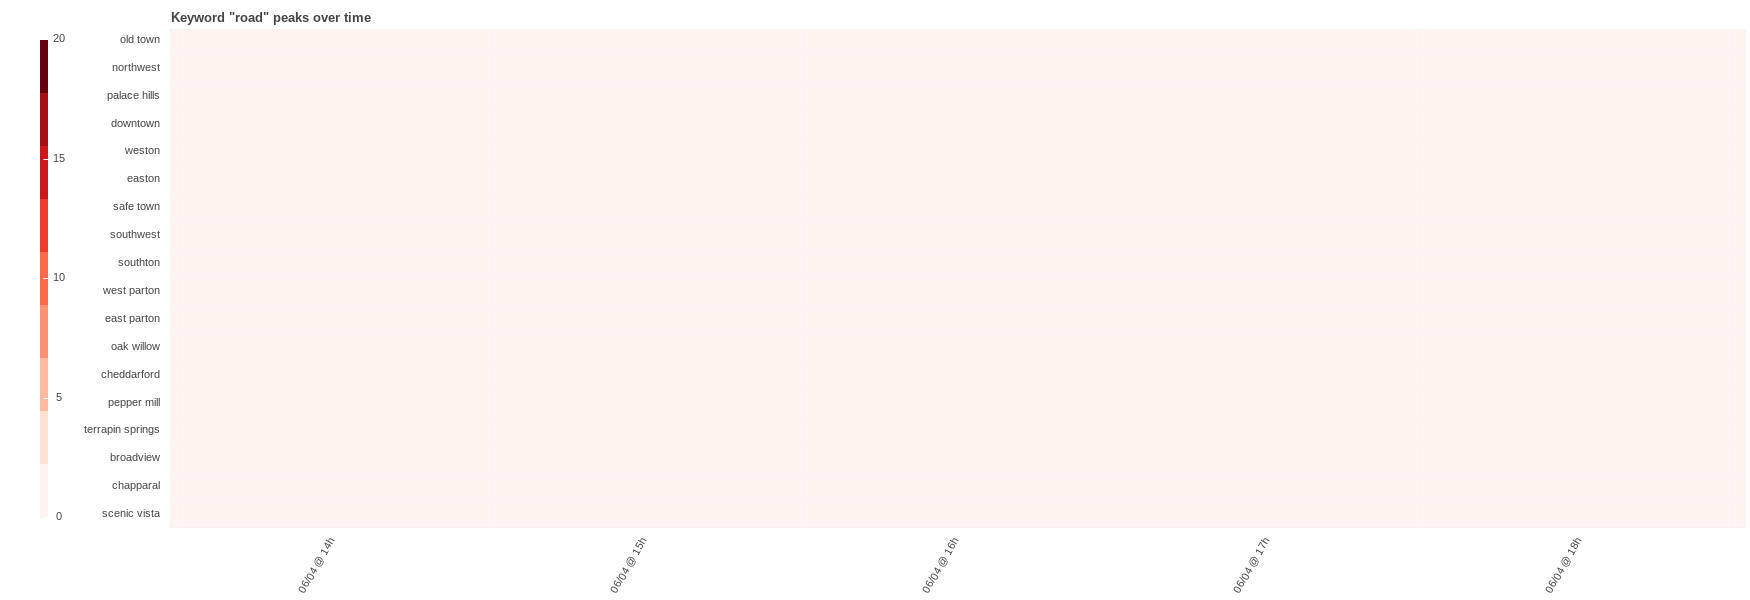
\includegraphics[width=1.00\textwidth]{figs/cond_5h/cond_5h_road.png}
        \caption{Roads and Bridges}
    \end{subfigure}
    \begin{subfigure}[!h]{0.32\textwidth}
        \centering
        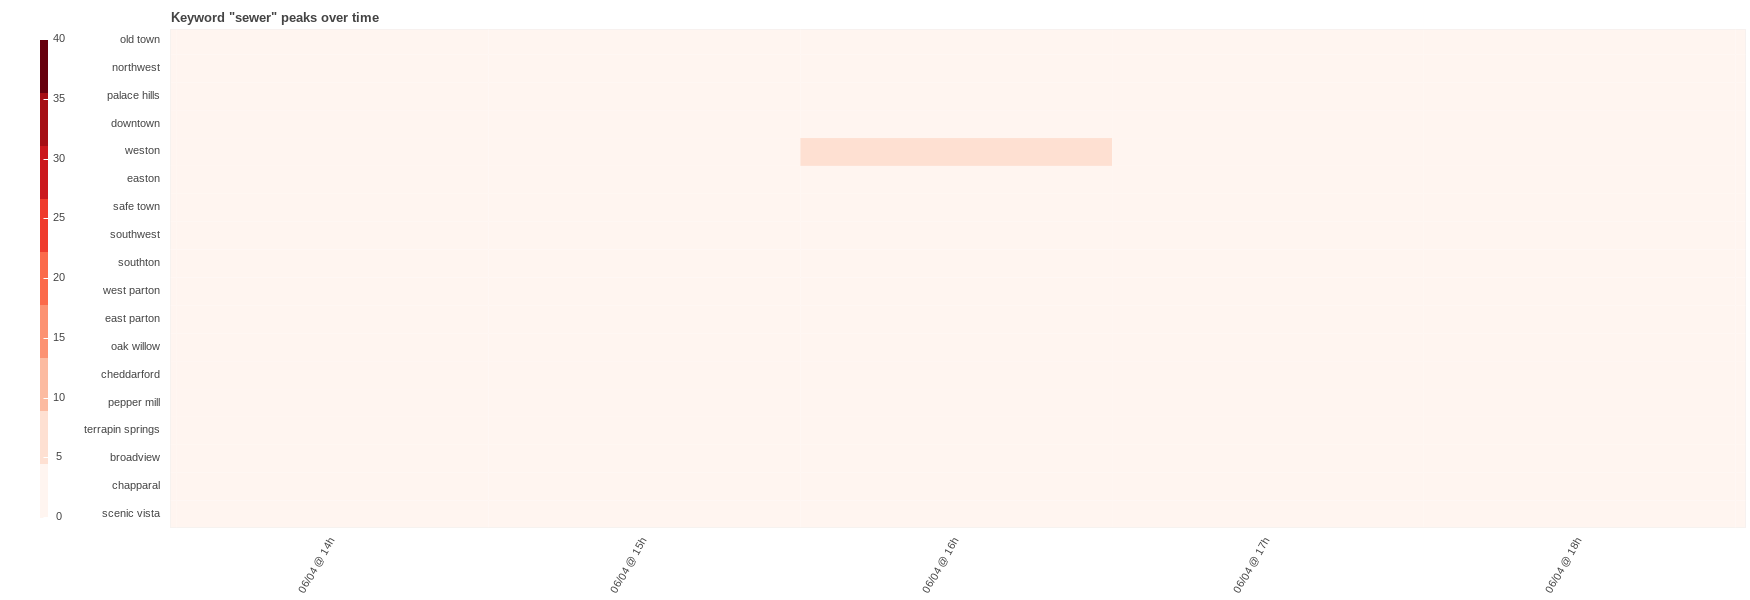
\includegraphics[width=1.00\textwidth]{figs/cond_5h/cond_5h_sewer.png}
        \caption{Sewer and water}
    \end{subfigure}
    \begin{subfigure}[!h]{0.32\textwidth}
        \centering
        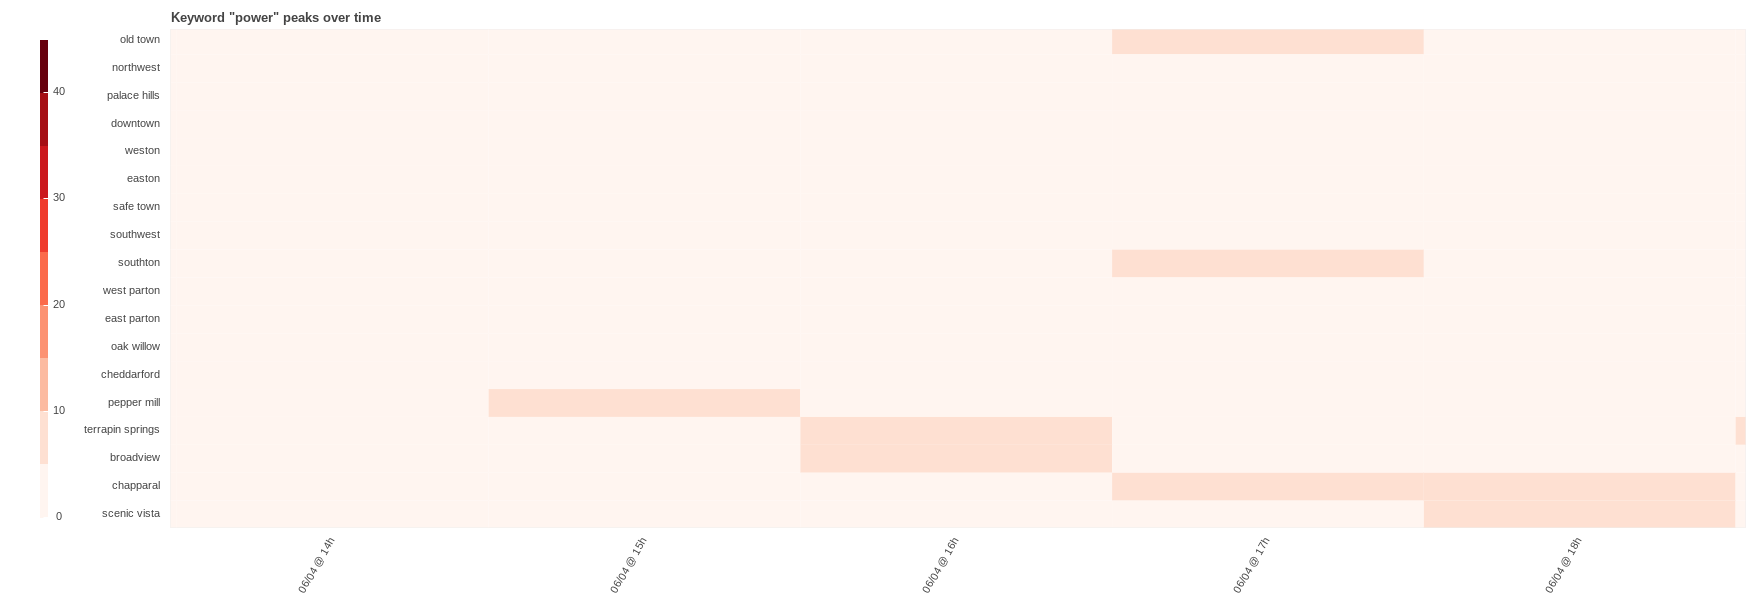
\includegraphics[width=1.00\textwidth]{figs/cond_5h/cond_5h_power.png}
        \caption{Power}
    \end{subfigure}
    \begin{subfigure}[!h]{0.32\textwidth}
        \centering
        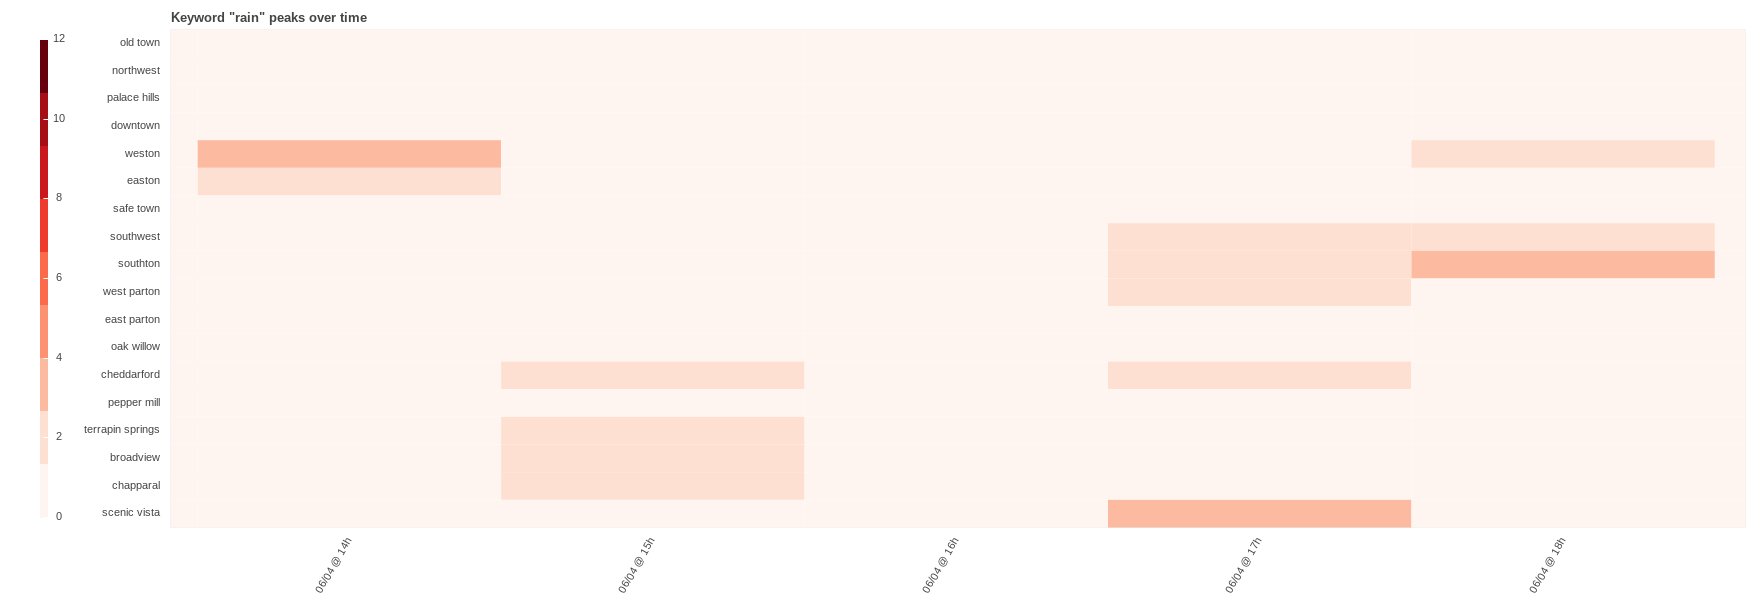
\includegraphics[width=1.00\textwidth]{figs/cond_5h/cond_5h_rain.png}
        \caption{Rain}
    \end{subfigure}
    \caption{Earthquake conditions after 5h}
    \label{fig:eq_cond_5h}
\end{figure}

Suggestions for crew allocation is detailed as follows: 

\begin{itemize}
    \item \emph{Sewer and water:} A crew must be sent only to Weston between 
    4:00~PM and 4:59~PM.
    \smallskip 
    \item \emph{Power}: Issues have occurred in Pepper Mill, \textbf{Terrapin
    Springs}, \textbf{Broadview}, Chapparal, \textbf{Southton}, \textbf{Old 
    Town} and Scenic Vista, but we'll consider only the locations 
    highlighted in bold because they have hospitals.
    \begin{itemize}
        \item A crew must be sent to Terrapin Springs between 3:00~PM and
        3:59~PM. Broadview also has a power demand at this time interval but the
        tweet frequency is much lower considering the five-hour period.
        \item Two crews must be sent to Old Town and Southton between 4:00~PM 
        and 4:59~PM.
        \item Lastly, the crew from Terrapin Springs can be reallocated to
        Chapparal between 5:00~PM and 5:59~PM. Although Chapparal does not have
        hospitals, it has been nearly two hours with electrical issues.
    \end{itemize}
    \item \emph{Rescue, sewer and water}: A crew must be sent to Southton only
    because there have been small issues in Weston, Southton and Downtown, and
    therefore Southton is geographically in the middle of such neighbourhoods.
\end{itemize}

\newpage

\subsection{How resources should be allocated 30h after the earthquake?}
Looking at the useful-words colormap over the SVG map of St. Hirmak, it can be
inferred right at the outset that the neighbourhoods that are in most need are
Downtown, Southton, Old Town and Weston.

\begin{figure}[!h]
    \centering
    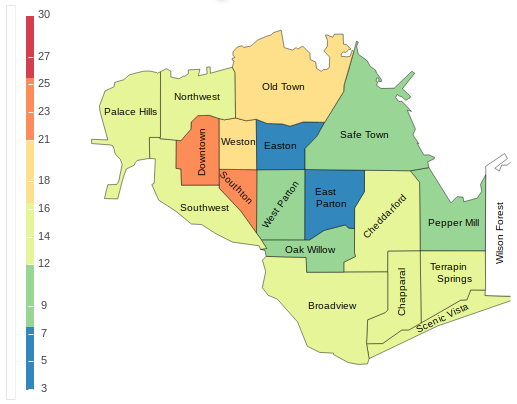
\includegraphics[width=0.30\textwidth]{figs/cond_30h/cond_30h_svg.png}
    \label{fig:map_30h}
    \caption{St. Himark's map 30h after the first earthquake.}
\end{figure}

By looking at the heatmap of Figure~\ref{fig:eq_cond_30h} for each keyword, it
can be seen that there have been no occurrences for medical, and the ones
related to sewer/water and rain have already been attended within the first five
hours. With respect to roads and bridges in particular, there have been 3
occurrences from 10:00~AM to 11:00~AM of April 8th at Downtown, but this
neighbourhood is under resurfacing maintenance, which implies a road crew is
already working there.

\begin{figure}[!h]
    \centering
    \begin{subfigure}[!h]{0.48\textwidth}
        \centering
        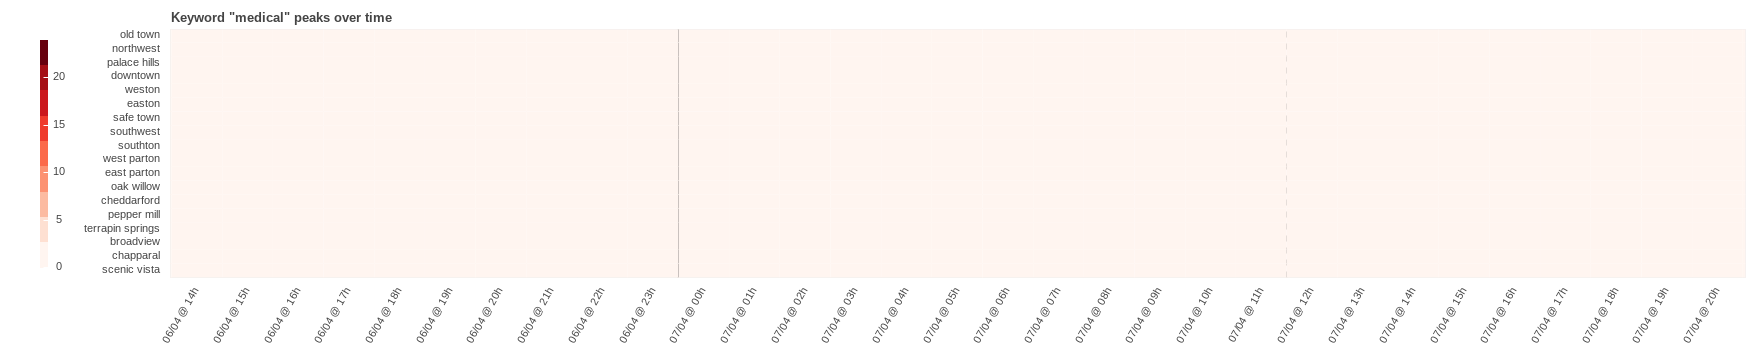
\includegraphics[width=1.00\textwidth]{figs/cond_30h/cond_30h_medical.png}
        \caption{Medical}
    \end{subfigure}
    \begin{subfigure}[!h]{0.48\textwidth}
        \centering
        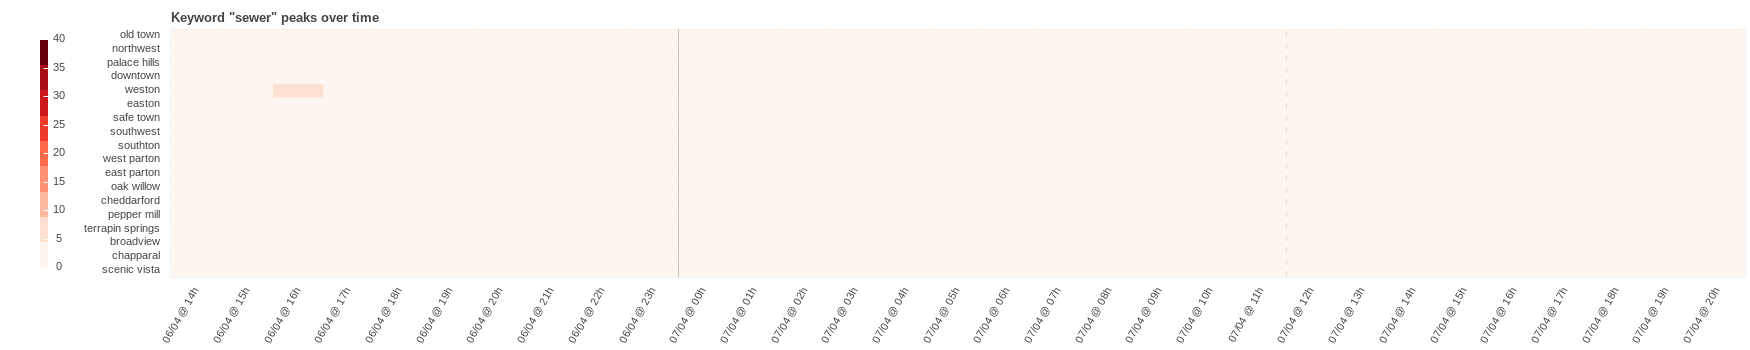
\includegraphics[width=1.00\textwidth]{figs/cond_30h/cond_30h_sewer.png}
        \caption{Sewer and water}
    \end{subfigure}
    \begin{subfigure}[!h]{0.48\textwidth}
        \centering
        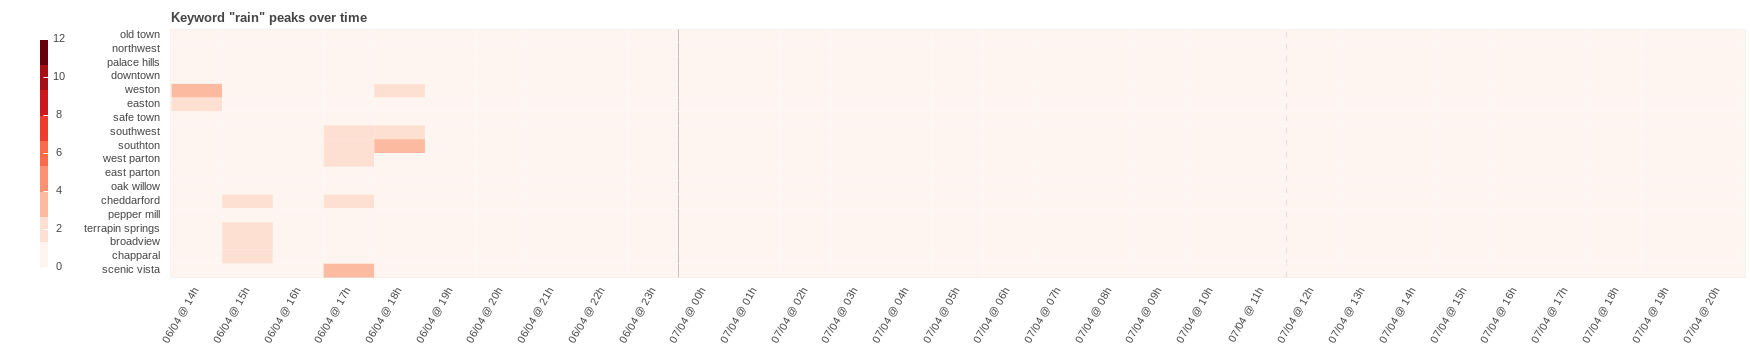
\includegraphics[width=1.00\textwidth]{figs/cond_30h/cond_30h_rain.png}
        \caption{Rain}
    \end{subfigure}
    \begin{subfigure}[!h]{0.48\textwidth}
        \centering
        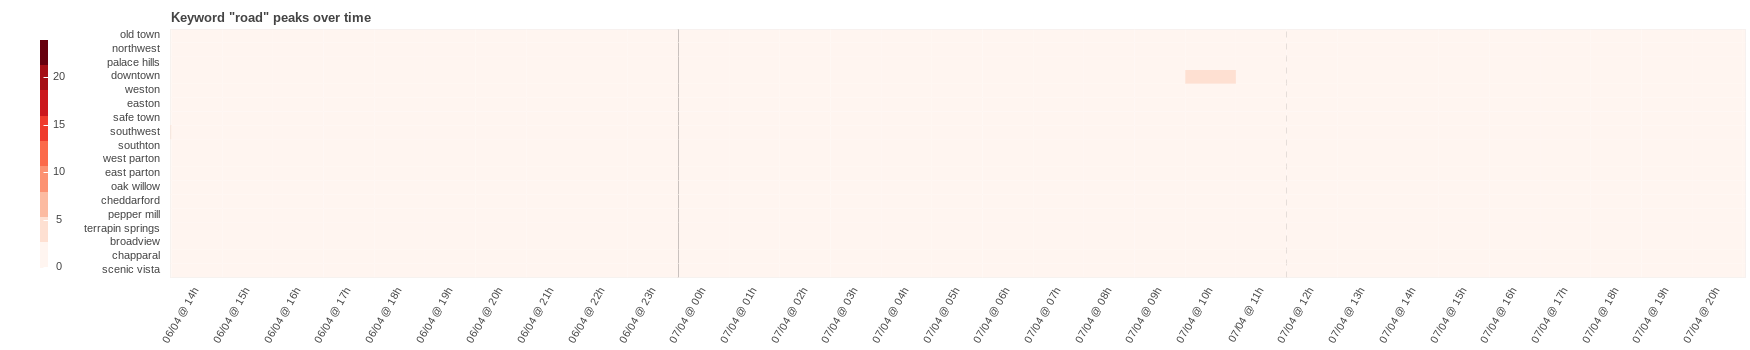
\includegraphics[width=1.00\textwidth]{figs/cond_30h/cond_30h_road.png}
        \caption{Roads and Bridges}
    \end{subfigure}
    \begin{subfigure}[!h]{0.48\textwidth}
        \centering
        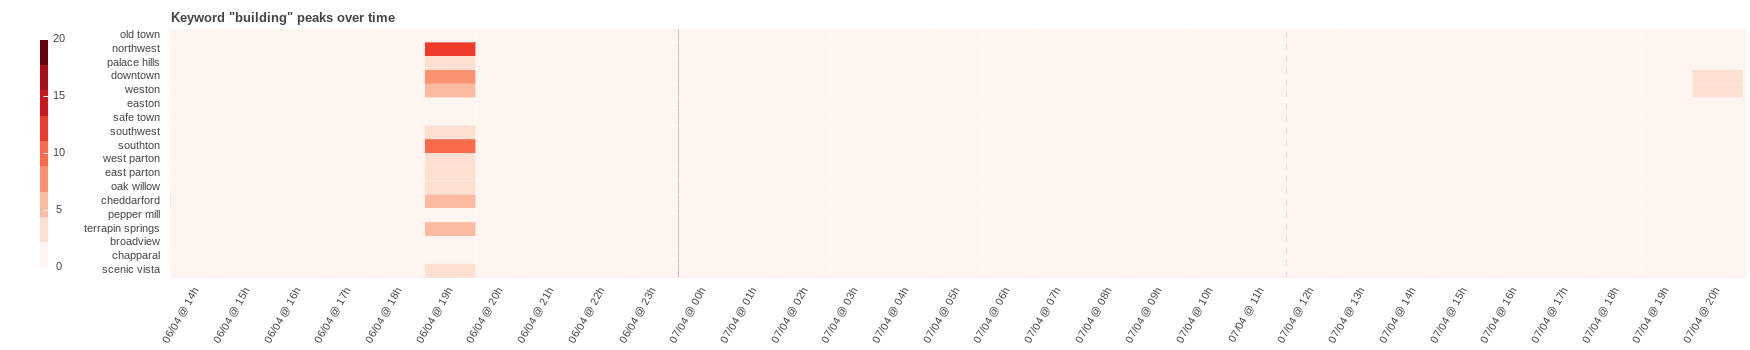
\includegraphics[width=1.00\textwidth]{figs/cond_30h/cond_30h_build.png}
        \caption{Building}
    \end{subfigure}
    \begin{subfigure}[!h]{0.48\textwidth}
        \centering
        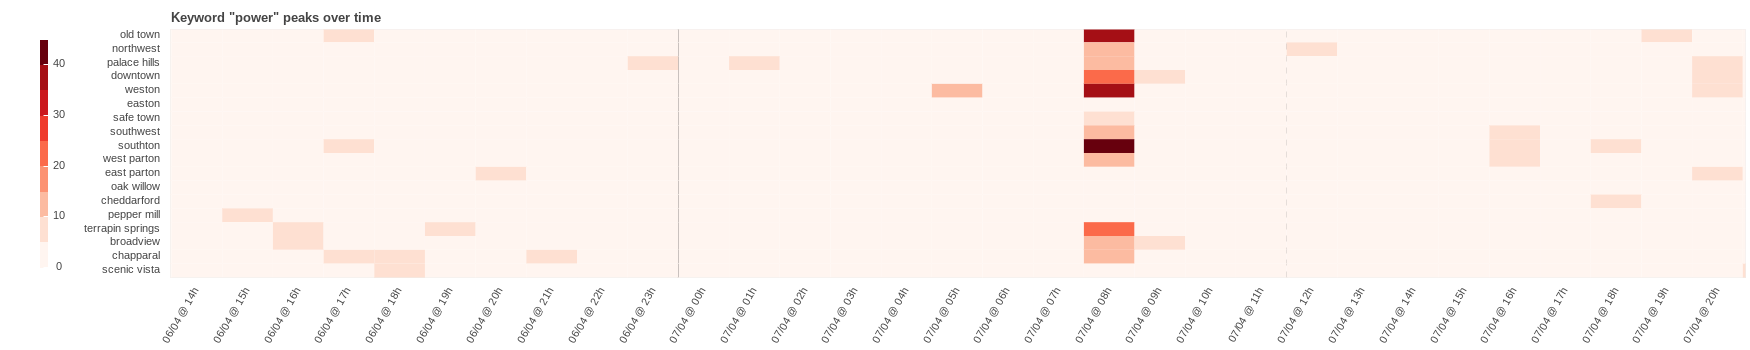
\includegraphics[width=1.00\textwidth]{figs/cond_30h/cond_30h_power.png}
        \caption{Power}
    \end{subfigure}
    \caption{Earthquake conditions after 30h}
    \label{fig:eq_cond_30h}
\end{figure}

Suggestions for crew allocation is detailed as follows:

\begin{itemize}
    \item \emph{Building}: On April 7th from 7:00~PM to 7:59~PM there have been
    multiple casualties on almost all locations so we would prioritize the
    dark-red-colored ones according to the heatmap of Figure~\ref{fig:eita}:
    Northwest, Southton, Downtown, and Weston. All four have a high 
    density of buildings and people, apart from being geographically close to
    each other, which can be an advantage for an eventual reallocation of crews
    in the following hours. Terrapin Springs and Cheddarford also have some
    less-intense occurrences, but they must be ignored due to the absence of
    high buildings.
    \item \emph{Power}: On April 7th there have been sporadic, less-intense
    occurrences that could be solved by sending small units to individual
    locations, but from 8:00~AM to 9:00~AM an energy disaster appear to have
    affected almost all neighbourhoods. Again we would prioritize regions where
    the keywords were mentioned the most: Southton, Old Town, and Weston. The
    other can be later attended in the following hours.
\end{itemize}
\end{section}

\begin{section}{Question}
\end{section}
\end{document}
